% Discussion

\chapter{Discussion}

With All these result the tune can be assumed to be visible and it is then possible to assess the feasability of the tune measurement using \gls{GPU}. There is still some question around hardware update but the work left to be done can be fairely well estimated.

\section{Observation}

During the three \gls{MD} we acquired around TODO with both beam and both planes. This data was acquired in XML files and stored on the \gls{CERN} infrastructure. XML was chosen as it is easily accessible by both custom and commercial data analysis software.

Matlab was used as the first tool to check the data and try different algorithm but in the end the software was ready fast enough and flexible enough. Matlab ended to be only used for check and test puprose and all the analysis and discussion is based on the result obtain with the data analysis software described in section \ref{sec:data_analysis_software}

	\subsection{Without damper}

	When the \gls{ADT} is off line there is a clear mark on the tune as shown on figure \ref{fig:adt_off}. There is still discution on is it the tune or just a ripple of the tune but as when the tune is moved the mark is also moving it is safe to assume this is really the tune. Some test could still be made, crosschecking with the \gls{BBQ}, changing the tune and looking in real time.

	\begin{figure}[H]
	\caption{Spectrogram with ADT off on the 16 October 2012 on vertical beam 1 before the ramp}
	\label{fig:adt_off}
	\centering
	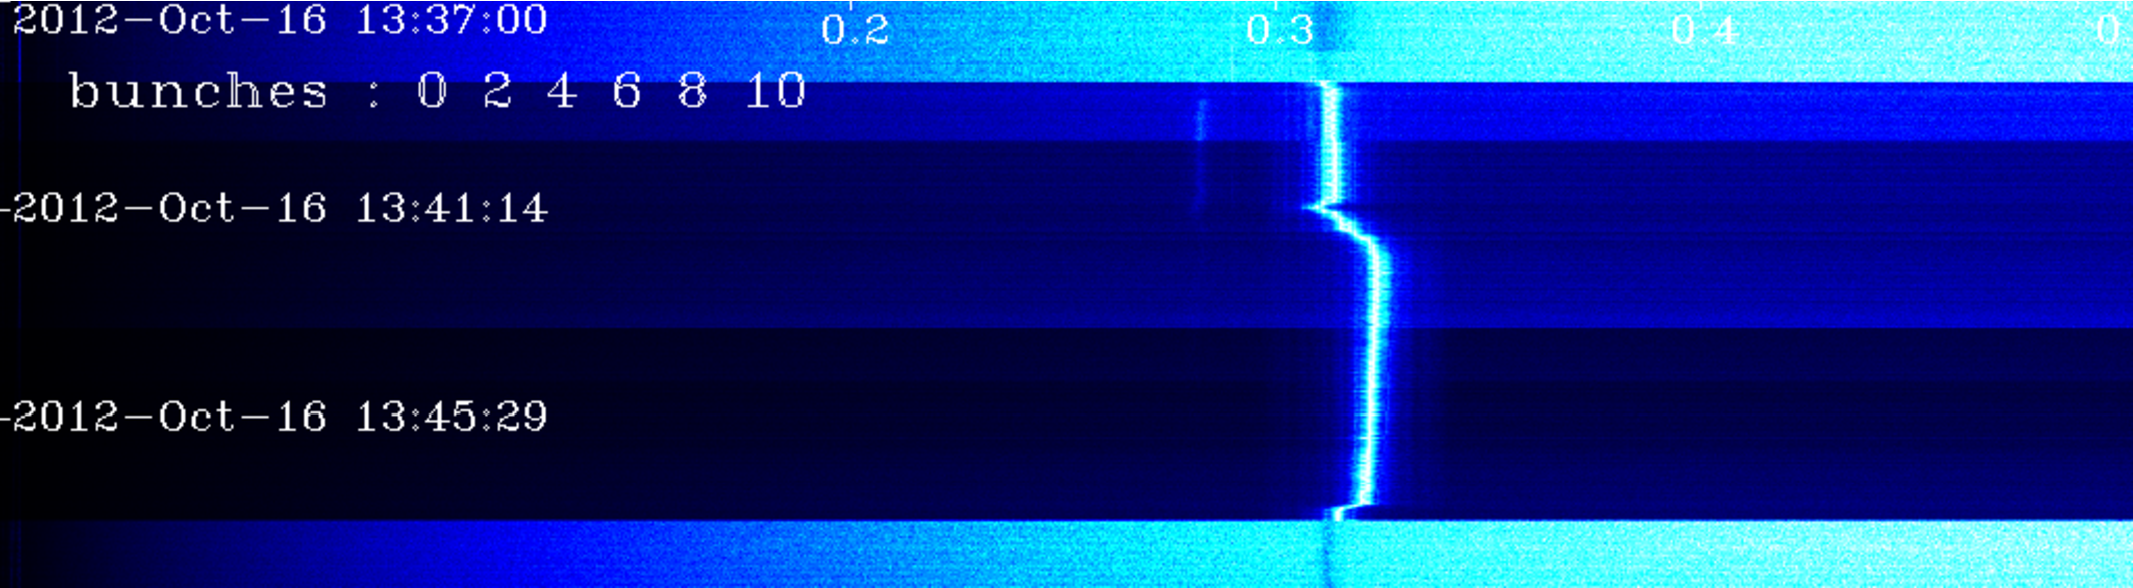
\includegraphics[scale=0.3]{md-121016-vb1-m1-6bunches-10acc-1337-1349-ADT-off.pdf}
	\end{figure}

	These observations are consistent with the gated-\gls{BBQ} result of 2012 \cite{Valuch12} and show that we can acquire the tune with the \gls{ADT} and get a clear bunch-by-bunch view of the tune even for only one bunch as shown in figure \ref{fig:one_bunch_adt_off}

	\subsection{With damper}

	\begin{figure}[H]
	\caption{Spectrogram with damper working on the 16 Octover 2012 on vertical beam 1 during the ramp}
	\centering
	\label{fig:ramp}
	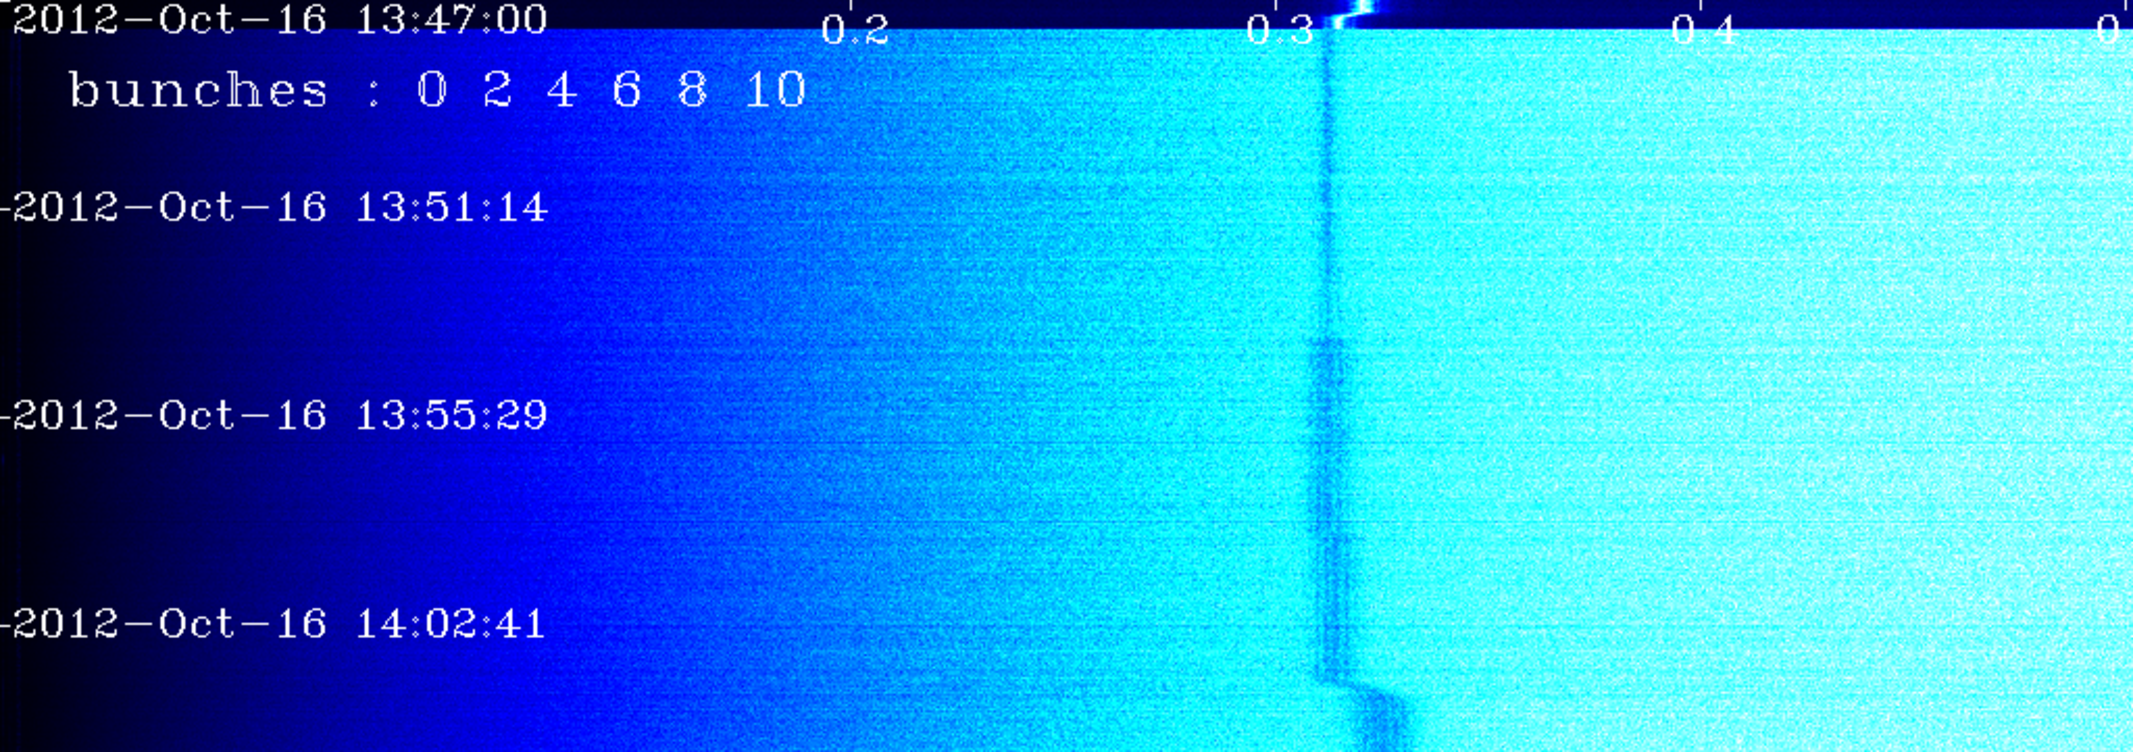
\includegraphics[scale=0.3]{md-121016-vb1-m1-6bunches-10acc-1347-1405-ramp.pdf}
	\end{figure}

	The tune is inverted speak about cite the hofle paper mathematic morphology more processing needed but should be quite low.

\section{Data flow}

\begin{figure}[H]
\caption{Acquisition data flow}
\centering
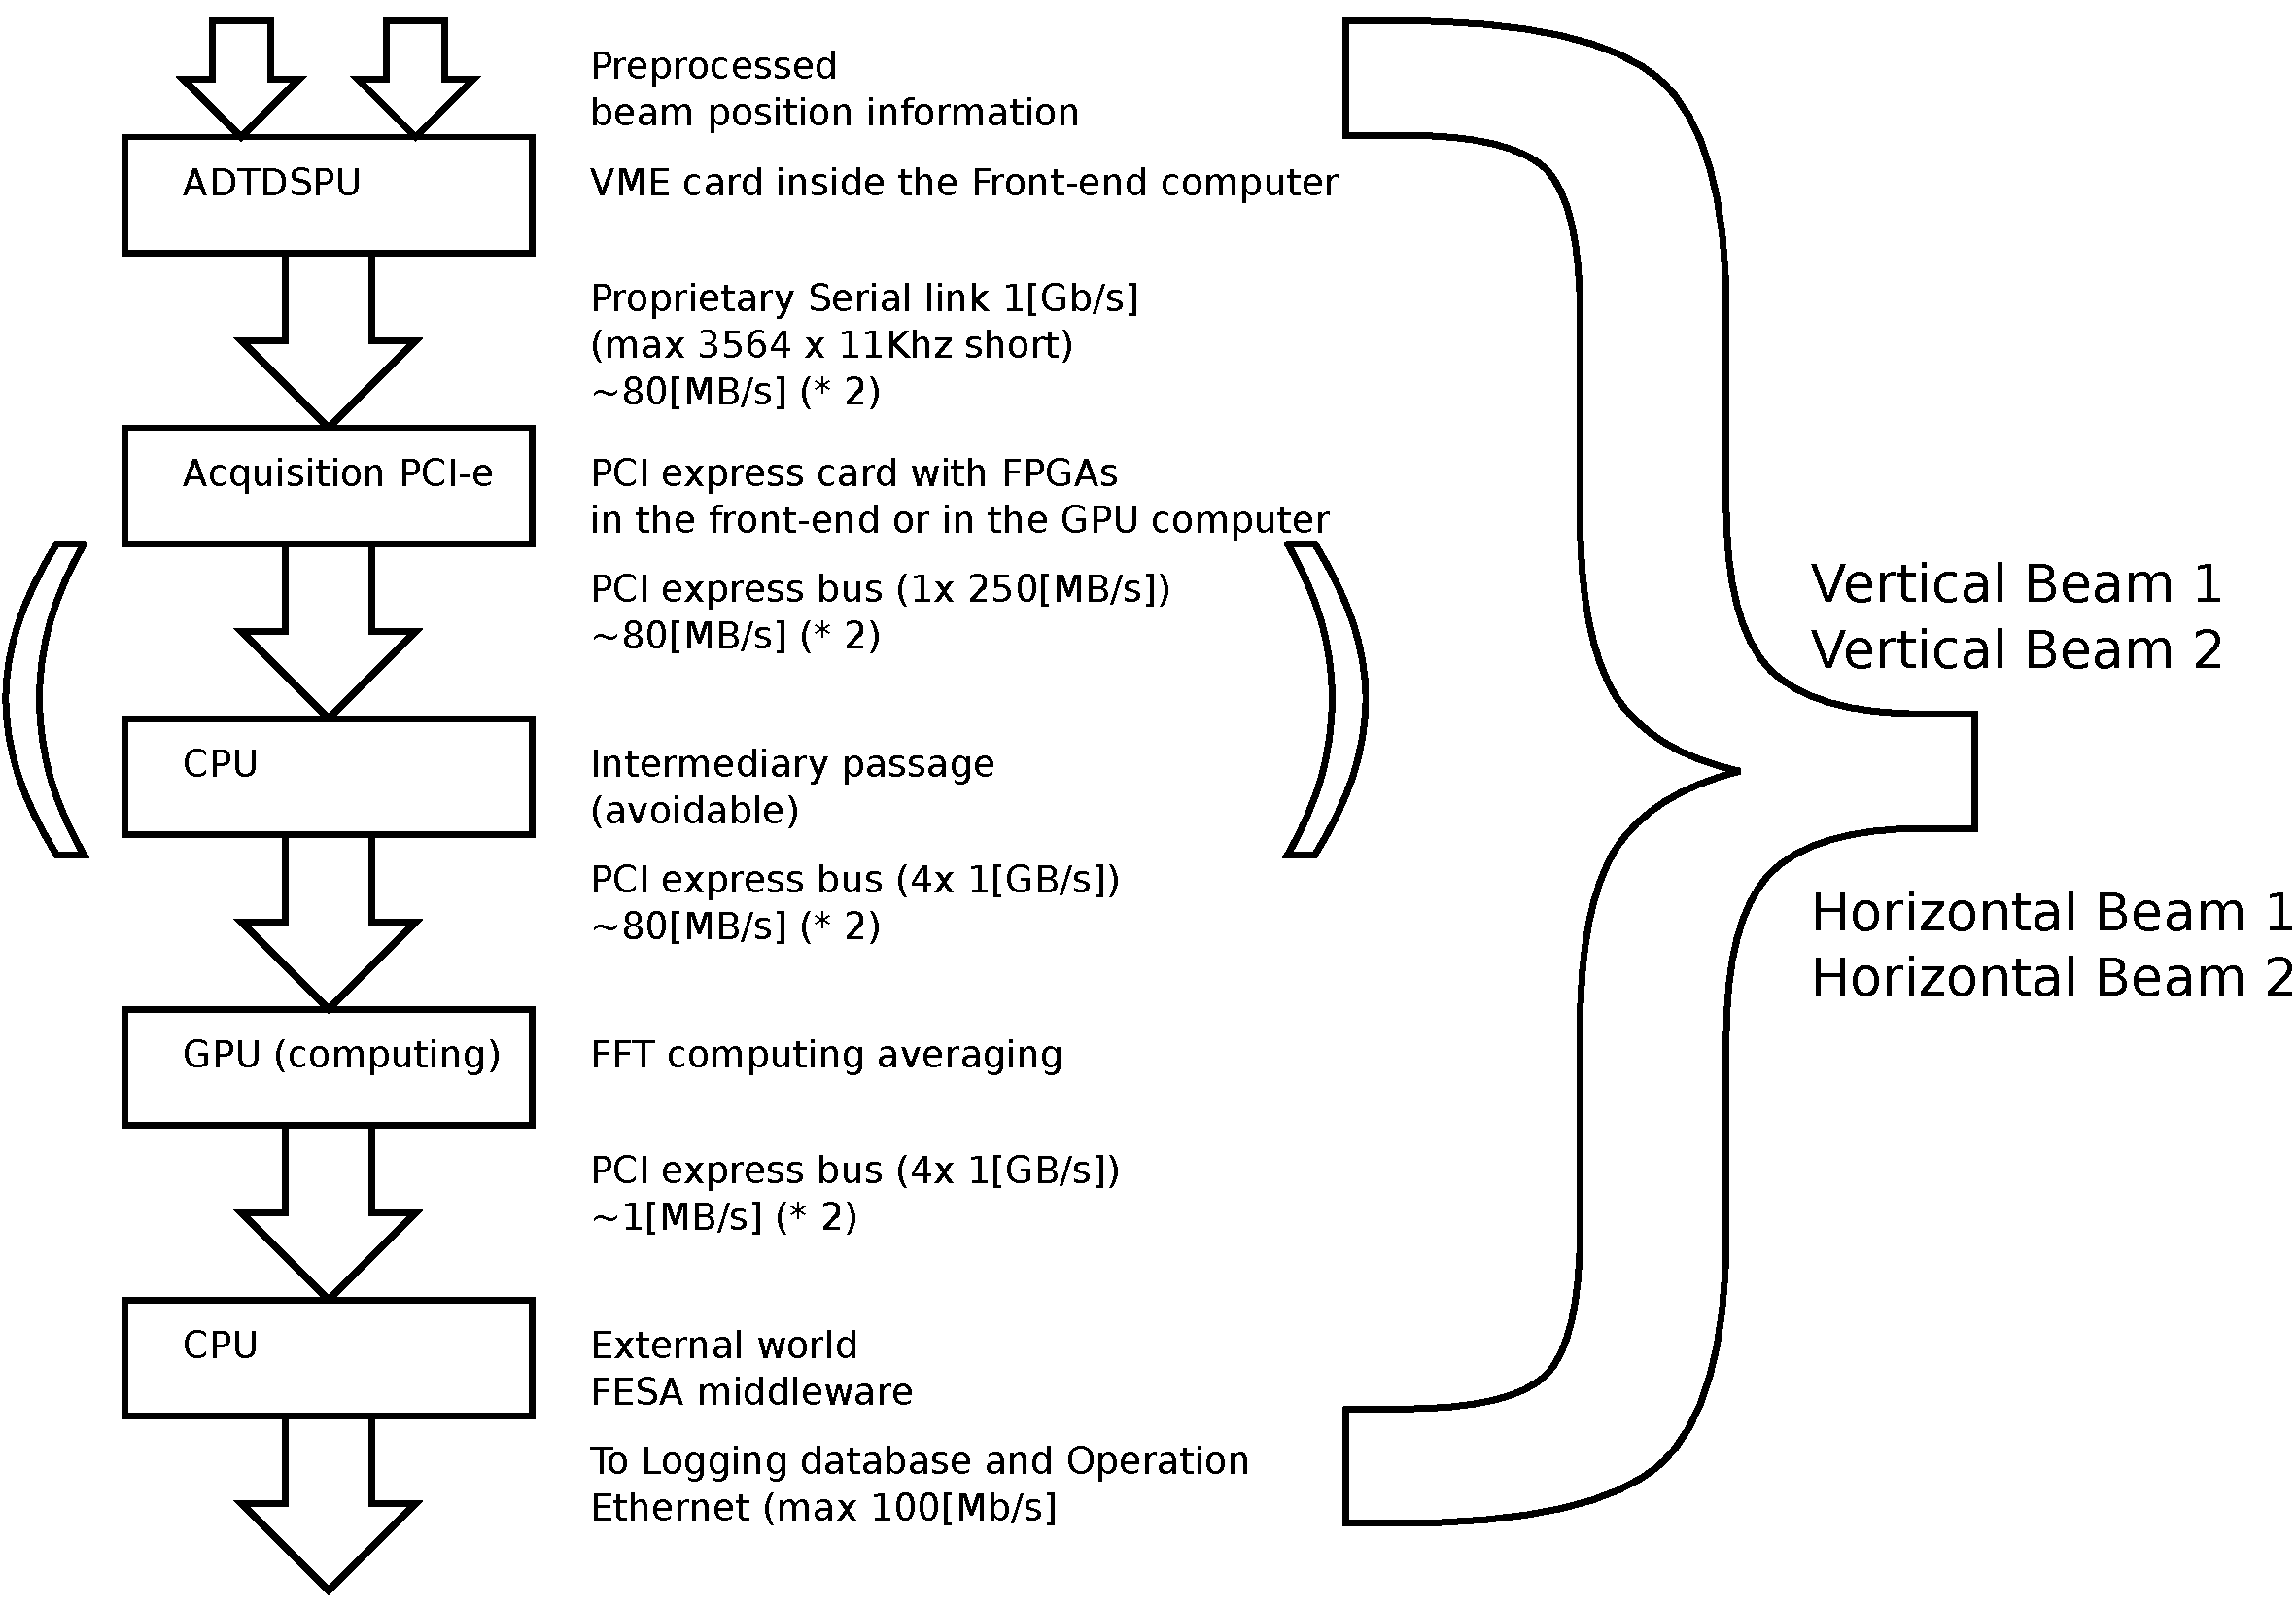
\includegraphics[scale=0.3]{dataflow.pdf}
\end{figure}

\section{Hardware}

	\subsection{ADT Aquisition boards}

	\subsection{Serial link interface}

	\subsection{GPUs}

\section{Software}

	\subsection{Drivers}

	\subsection{OpenCL}

	\subsection{Front-end}

\section{Estimated Cost}